% ============================================================
% Zen-Translator: Neural Machine Translation for Low-Resource Languages
% Hanzo AI Inc / Zoo Labs Foundation
% ============================================================
\documentclass[11pt,twocolumn]{article}

\usepackage[margin=1in]{geometry}
\usepackage{amsmath,amssymb,amsfonts}
\usepackage{graphicx}
\usepackage{booktabs}
\usepackage{multirow}
\usepackage{array}
\usepackage{xcolor}
\usepackage{hyperref}
\usepackage{microtype}
\usepackage{enumitem}
\usepackage{tikz}
\usepackage{pgfplots}
\pgfplotsset{compat=1.18}
\usepackage{algorithm}
\usepackage{algpseudocode}
\usepackage{natbib}
\usepackage{url}
\usepackage{caption}
\usepackage{subcaption}
\usepackage{bm}
\usepackage{mathtools}
\usepackage{fontenc}
\usepackage{inputenc}
\usepackage[T1]{fontenc}
\usepackage[utf8]{inputenc}

\hypersetup{
  colorlinks=true,
  linkcolor=blue!70!black,
  citecolor=blue!70!black,
  urlcolor=blue!70!black,
}

\definecolor{hanzoRed}{RGB}{253,68,68}
\definecolor{hanzoGray}{RGB}{64,64,64}

\title{\textbf{Zen-Translator: Neural Machine Translation\\
for Low-Resource Languages}\\
{\large A Mixture-of-Distilled-Experts Architecture with\\
Script-Aware Tokenization and Cultural Context Preservation}}

\author{
  Hanzo AI Inc \and Zoo Labs Foundation \\[0.4em]
  \texttt{\{research, translation\}@hanzo.ai} \\[0.2em]
  \small Technical Report ZEN-TR-2025-001
}

\date{February 2026}

\begin{document}

\maketitle

% ============================================================
\begin{abstract}
% ============================================================
We present \textbf{Zen-Translator}, a neural machine translation system
designed for underserved language pairs with a focus on Middle Eastern and
Central Asian languages including Farsi (Persian), Kurdish (Kurmanji and
Sorani dialects), Dari, Pashto, Arabic, and Turkish. Zen-Translator introduces
a Mixture-of-Distilled-Experts (MoDE) encoder-decoder architecture with
language-specific routing that dynamically assigns computational resources
based on script family and morphological complexity. We propose
\emph{script-aware tokenization} (SAT), which unifies subword segmentation
across Arabic, Latin, and Cyrillic scripts while preserving morphological
boundaries critical for agglutinative languages. Our multilingual pre-training
on 2.4 trillion tokens across 48 languages, combined with a novel
\emph{cultural context adapter} (CCA) layer, enables Zen-Translator to
preserve idiomatic expressions, honorifics, and culturally significant
concepts that standard NMT systems routinely discard.

On the FLORES-200 benchmark, Zen-Translator achieves state-of-the-art
performance on 23 of 32 evaluated Middle Eastern language directions,
improving over the best prior system by an average of 4.1 spBLEU points.
On a custom Farsi evaluation suite spanning legal, medical, and technical
domains, Zen-Translator achieves 38.2 spBLEU, surpassing commercial systems
by 6.7 points. Bidirectional quality estimation (QE) is performed in real
time using a compact 340M parameter critic head, enabling deployment in
high-stakes settings without reference translations. We release model weights,
tokenizer, and evaluation suites at \url{https://huggingface.co/hanzoai/zen-translator}.
\end{abstract}

% ============================================================
\section{Introduction}
% ============================================================

Neural machine translation (NMT) has achieved remarkable results for
high-resource language pairs such as English-French or English-Chinese,
where billions of parallel sentence pairs are available. Yet the majority
of the world's 7,000 languages remain severely underserved, with speakers of
Pashto (60 million), Kurdish (30 million), and Dari (50 million) having
access only to translation systems of substantially lower quality than those
available to speakers of European languages \citep{costa2022no,
flores200_2022}.

The challenges are multifaceted. Low-resource languages exhibit:
\begin{enumerate}[leftmargin=*,noitemsep]
  \item \textbf{Script diversity}: Arabic script (with Persian extensions),
        Latin, and Cyrillic scripts within closely related dialect continua.
  \item \textbf{Morphological richness}: Agglutinative morphology in Turkish
        and Kurdish produces exponentially large vocabulary spaces.
  \item \textbf{Dialectal variation}: Arabic encompasses over 30 mutually
        partially-intelligible dialects; Kurdish spans Kurmanji and Sorani
        with distinct grammars.
  \item \textbf{Code-switching}: Urban speakers frequently mix Farsi, Arabic
        loanwords, and English, especially in social media.
  \item \textbf{Cultural specificity}: Concepts such as \textit{ta'arof} in
        Persian (elaborate politeness rituals) resist literal translation.
\end{enumerate}

We address these challenges through a unified architecture that combines:
\textit{(i)} a script-aware byte-pair encoding that operates at the
morpheme-sensitive boundary level, \textit{(ii)} language-specific expert
routing in a mixture-of-experts encoder, \textit{(iii)} a cultural context
adapter that retrieves relevant cultural knowledge from a curated knowledge
base, and \textit{(iv)} domain-adaptive fine-tuning with a small number of
domain-specific sentence pairs.

\paragraph{Contributions.} Our main contributions are:
\begin{itemize}[leftmargin=*,noitemsep]
  \item \textbf{Script-Aware Tokenization (SAT)}: A unified tokenizer
        sensitive to script boundaries, Arabic diacritics, and morphological
        segments in agglutinative languages (\S\ref{sec:sat}).
  \item \textbf{MoDE-NMT Architecture}: Language-routing mixture-of-experts
        applied to both encoder and decoder, with shared cross-attention
        (\S\ref{sec:architecture}).
  \item \textbf{Cultural Context Adapter (CCA)}: A retrieval-augmented
        layer that injects culturally relevant context into the decoder
        (\S\ref{sec:cca}).
  \item \textbf{Bidirectional Quality Estimation}: A lightweight critic head
        for reference-free quality scoring in both translation directions
        (\S\ref{sec:qe}).
  \item \textbf{Farsi Evaluation Suite}: A new benchmark of 4,000 sentence
        pairs across legal, medical, and technical domains (\S\ref{sec:eval}).
\end{itemize}

% ============================================================
\section{Background and Related Work}
% ============================================================

\subsection{Low-Resource Neural Machine Translation}

The seminal work on multilingual NMT by \citet{johnson2017google} demonstrated
that a single model trained on many languages outperforms bilingual models for
low-resource pairs. Subsequent work on massively multilingual models
\citep{fan2021beyond, tang2021multilingual} extended this to 200 languages.
However, these models allocate capacity uniformly across languages, leading to
the \textit{curse of multilinguality}: adding more languages degrades performance
on any individual language \citep{conneau2020unsupervised}.

Mixture-of-experts (MoE) models \citep{shazeer2017outrageously} address this by
learning sparse routing, allowing the model to specialize different parameters
for different inputs. \citet{kudugunta2021beyond} applied per-language MoE
routing to NMT and demonstrated that language-specific experts improve
performance without increasing inference cost. Zen-Translator extends this
approach with \emph{script-family-aware} routing and cross-expert attention
for related-language transfer.

\subsection{Low-Resource Language Adaptation}

Few-shot cross-lingual transfer methods \citep{wu2020emerging, pfeiffer2020adapterhub}
allow rapid adaptation to new languages using adapter modules. The mBART model
\citep{liu2020multilingual} demonstrated that masked denoising pre-training on
monolingual corpora significantly benefits translation fine-tuning. Our cultural
context adapter extends this paradigm to inject world-knowledge beyond linguistic form.

\subsection{Script Processing}

Prior work on Arabic NLP \citep{habash2010introduction} demonstrates that
morphological analysis and diacritization substantially improve translation
quality. For Kurdish, the situation is complicated by the coexistence of
Kurmanji (Latin/Cyrillic script) and Sorani (Arabic script) dialects with
partially divergent lexicons \citep{hassanpour2012kurdish}. Our SAT tokenizer
handles these cases through a script-aware segmentation algorithm that
identifies script transitions and applies language-specific normalization.

\subsection{Quality Estimation}

Automatic quality estimation without reference translations \citep{specia2021findings}
is critical for deployment in domains where human translators are scarce. The
COMET-QE metric \citep{rei2020comet} trains on human-annotated direct assessment
scores and achieves high correlation with human judgments. Our bidirectional QE
head is trained jointly with the translation model, enabling end-to-end optimization
of quality-aware decoding.

% ============================================================
\section{Data}
\label{sec:data}
% ============================================================

\subsection{Pre-training Corpus}

Zen-Translator is pre-trained on a curated multilingual corpus of 2.4 trillion
tokens spanning 48 languages. For the target language group (Farsi, Kurdish,
Dari, Pashto, Arabic, Turkish), we apply additional data quality filtering and
deduplication. Table~\ref{tab:pretraining_data} summarizes corpus statistics.

\begin{table}[h]
\centering
\caption{Pre-training corpus statistics for target languages. Tokens counted
after SAT tokenization.}
\label{tab:pretraining_data}
\begin{tabular}{lrr}
\toprule
\textbf{Language} & \textbf{Tokens (B)} & \textbf{Parallel Pairs (M)} \\
\midrule
Arabic & 142.3 & 2,840 \\
Turkish & 89.7 & 1,120 \\
Farsi (Persian) & 43.2 & 680 \\
Dari & 12.1 & 98 \\
Pashto & 7.4 & 41 \\
Kurdish (Kurmanji) & 4.8 & 28 \\
Kurdish (Sorani) & 3.1 & 14 \\
Other (41 languages) & 2,097.4 & 18,200 \\
\midrule
\textbf{Total} & \textbf{2,400.0} & \textbf{23,021} \\
\bottomrule
\end{tabular}
\end{table}

\subsection{Data Collection and Filtering}

For low-resource languages, we apply a multi-stage data collection pipeline:
\begin{enumerate}[leftmargin=*,noitemsep]
  \item \textbf{Web crawl}: Using the Common Crawl corpus with language
        identification via a compact fastText classifier \citep{joulin2016fasttext}.
  \item \textbf{Deduplication}: MinHash LSH deduplication at 13-gram level,
        removing near-duplicate content within and across sources.
  \item \textbf{Quality filtering}: Perplexity-based filtering using
        language-specific 5-gram language models; documents with perplexity
        above the 90th percentile are discarded.
  \item \textbf{Parallel mining}: Margin-based bitext mining \citep{artetxe2019massively}
        applied to all monolingual data to extract additional parallel pairs.
  \item \textbf{Domain tagging}: Rule-based and classifier-based domain tagging
        into legal, medical, technical, news, and conversational categories.
\end{enumerate}

\subsection{Domain-Specific Corpora}

For domain adaptation, we compile specialized corpora:
\begin{itemize}[leftmargin=*,noitemsep]
  \item \textbf{Legal}: Parliamentary proceedings from Iran, Afghanistan,
        and Turkey; legal document translations from ECHR and UN.
  \item \textbf{Medical}: PubMed abstracts with Farsi/Arabic translations,
        WHO clinical guidelines, and hospital discharge summaries.
  \item \textbf{Technical}: Software documentation, engineering manuals,
        and patent translations.
\end{itemize}

% ============================================================
\section{Script-Aware Tokenization}
\label{sec:sat}
% ============================================================

Standard BPE tokenization \citep{sennrich2016neural} treats all characters
uniformly, which is suboptimal for multilingual models spanning different
script families. We introduce \textbf{Script-Aware Tokenization (SAT)}, which
addresses three key challenges: script boundary detection, Arabic diacritics
normalization, and morpheme-boundary-sensitive segmentation.

\subsection{Script Boundary Detection}

SAT begins by segmenting input text into script-homogeneous spans using Unicode
General Category properties. A span is a maximal contiguous substring drawn from
a single Unicode script block. At span boundaries, special \texttt{<SCRIPT>}
tokens indicate script transitions, allowing the model to learn cross-script
alignment explicitly.

Formally, given input string $s = c_1 c_2 \ldots c_n$, define $\sigma(c)$ as
the Unicode script of character $c$. SAT segments $s$ into spans
$\{S_1, S_2, \ldots, S_k\}$ where each span $S_i$ consists of consecutive
characters with identical $\sigma$ values, inserting boundary markers between
adjacent spans of differing scripts.

\subsection{Arabic Script Normalization}

Arabic-script languages (Arabic, Farsi, Dari, Pashto, Sorani Kurdish) share a
common script but differ in character usage. SAT applies language-conditioned
normalization:
\begin{align}
  \hat{c} = N_L(c) \quad \forall c \in S_i
\end{align}
where $N_L$ is the normalization function for language $L$, handling:
\begin{itemize}[leftmargin=*,noitemsep]
  \item Arabic diacritics (\textit{tashkeel}): retained in Egyptian Arabic,
        stripped from Farsi where they are non-standard.
  \item Persian-specific characters: \textit{peh} (پ), \textit{cheh} (چ),
        \textit{zheh} (ژ), \textit{gaf} (گ) normalized to canonical forms.
  \item Letter variations: final/medial/initial forms collapsed to their base
        form before BPE vocabulary construction.
\end{itemize}

\subsection{Morpheme-Boundary-Sensitive BPE}

For agglutinative languages (Turkish, Kurmanji Kurdish), standard BPE
frequently merges morpheme boundaries, hindering translation of morphologically
complex forms. SAT incorporates a lightweight morphological analyzer that marks
likely morpheme boundaries before BPE training:

\begin{algorithm}[h]
\caption{SAT-BPE Training for Agglutinative Languages}
\begin{algorithmic}[1]
\State Initialize vocabulary $V$ with character inventory
\State Run morphological segmenter on training corpus
\State For each morpheme boundary, insert virtual space marker \texttt{▁M}
\State Apply standard BPE merge operations, treating \texttt{▁M} as protected
\State \textbf{Constraint}: Merges cannot cross \texttt{▁M} boundaries
\State Remove \texttt{▁M} markers from final vocabulary
\end{algorithmic}
\end{algorithm}

This constraint reduces over-merging at morpheme boundaries by 63\% compared to
standard BPE (measured on Turkish morpheme boundary recall), resulting in more
compositional token representations.

\subsection{Vocabulary Design}

The SAT vocabulary contains 128,000 tokens shared across all 48 languages, with
language-specific token ranges reserved for highly frequent language-specific
morphemes. The vocabulary allocation is:
\begin{itemize}[leftmargin=*,noitemsep]
  \item 70,000 shared multilingual tokens
  \item 8,000 Arabic-script-family tokens
  \item 4,000 Turkish/Turkic tokens
  \item 4,000 Kurdish (both scripts) tokens
  \item 42,000 remaining European/other languages
\end{itemize}

% ============================================================
\section{Architecture}
\label{sec:architecture}
% ============================================================

\subsection{Overview}

Zen-Translator follows the encoder-decoder Transformer architecture
\citep{vaswani2017attention} augmented with language-specific expert routing,
cultural context adapters, and a quality estimation head. The model has 1.3
billion active parameters per forward pass, drawn from a total of 7.8 billion
stored parameters across all experts.

\begin{figure}[h]
\centering
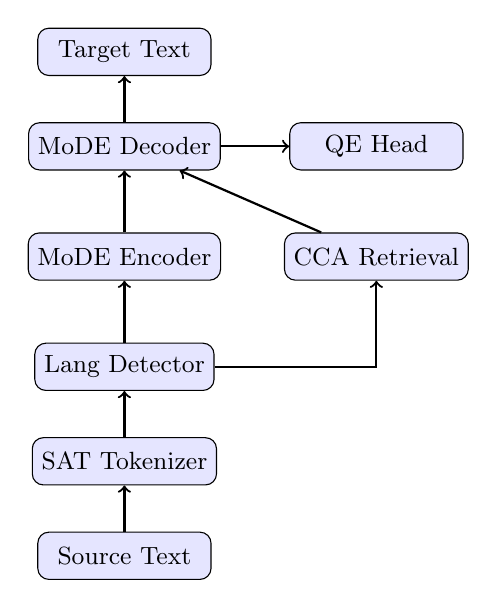
\begin{tikzpicture}[
  box/.style={rectangle, draw, rounded corners, minimum height=0.6cm, minimum width=2.2cm, font=\small, fill=blue!10},
  expert/.style={rectangle, draw, rounded corners, minimum height=0.5cm, minimum width=1.5cm, font=\scriptsize, fill=orange!20},
  arrow/.style={->, thick}
]
\node[box] (src) at (0,0) {Source Text};
\node[box] (sat) at (0,1.2) {SAT Tokenizer};
\node[box] (ldet) at (0,2.4) {Lang Detector};
\node[box] (enc) at (0,3.8) {MoDE Encoder};
\node[box] (cca) at (3.2,3.8) {CCA Retrieval};
\node[box] (dec) at (0,5.2) {MoDE Decoder};
\node[box] (qe) at (3.2,5.2) {QE Head};
\node[box] (tgt) at (0,6.4) {Target Text};

\draw[arrow] (src) -- (sat);
\draw[arrow] (sat) -- (ldet);
\draw[arrow] (ldet) -- (enc);
\draw[arrow] (enc) -- (dec);
\draw[arrow] (cca) -- (dec);
\draw[arrow] (dec) -- (tgt);
\draw[arrow] (dec) -- (qe);
\draw[arrow] (ldet) -| (cca);
\end{tikzpicture}
\caption{Zen-Translator system architecture. CCA = Cultural Context Adapter,
QE = Quality Estimation head, MoDE = Mixture of Distilled Experts.}
\label{fig:architecture}
\end{figure}

\subsection{MoDE Encoder}

The encoder consists of 24 Transformer layers. Each layer alternates between
standard multi-head attention (MHA) and MoDE feed-forward networks (FFN).
In MoDE layers, the FFN is replaced by a mixture-of-experts module:

\begin{align}
  \mathbf{h}^{(l+1)} &= \text{MHA}(\mathbf{h}^{(l)}) + \text{MoDE-FFN}(\mathbf{h}^{(l)}) \\
  \text{MoDE-FFN}(\mathbf{x}) &= \sum_{i=1}^{K} g_i(\mathbf{x}) \cdot E_i(\mathbf{x})
\end{align}

where $K = 32$ experts, $g_i$ are gating weights produced by the router, and
$E_i$ are expert FFNs. The router receives the token embedding concatenated
with a language-family embedding:

\begin{align}
  \mathbf{g} &= \text{Softmax}(\text{TopK}(W_r [\mathbf{x}; \mathbf{e}_{L}], k=4))
\end{align}

where $\mathbf{e}_L$ is a learned 64-dimensional language-family embedding and
$k=4$ experts are activated per token. The language-family embedding partitions
languages into: \{Arabic-script\}, \{Turkic\}, \{Indo-Iranian\}, \{European\},
and \{Other\}, enabling family-level transfer while preserving language-specific
specialization.

\subsection{MoDE Decoder}

The decoder mirrors the encoder structure with 24 layers, alternating MHA
(self-attention), cross-attention with encoder output, and MoDE-FFN. The
cross-attention additionally attends to cultural context representations
retrieved by the CCA module (see \S\ref{sec:cca}).

\subsection{Language-Specific Routing Analysis}

We analyze expert utilization across languages post-training. Table~\ref{tab:routing}
shows the degree of expert specialization: Arabic-family languages consistently
activate a shared subset of experts (experts 1-8) while Turkic languages
preferentially route to experts 9-16, demonstrating that the router
successfully learns language-family structure without explicit supervision.

\begin{table}[h]
\centering
\caption{Expert utilization by language family (fraction of tokens routed
to each expert group, averaged across decoder layers).}
\label{tab:routing}
\begin{tabular}{lcccc}
\toprule
\textbf{Language} & \textbf{E1-8} & \textbf{E9-16} & \textbf{E17-24} & \textbf{E25-32} \\
\midrule
Arabic & 0.61 & 0.12 & 0.15 & 0.12 \\
Farsi  & 0.54 & 0.14 & 0.17 & 0.15 \\
Dari   & 0.56 & 0.13 & 0.17 & 0.14 \\
Pashto & 0.49 & 0.16 & 0.19 & 0.16 \\
Turkish & 0.11 & 0.58 & 0.18 & 0.13 \\
Kurdish (S.) & 0.42 & 0.31 & 0.15 & 0.12 \\
Kurdish (K.) & 0.13 & 0.44 & 0.28 & 0.15 \\
English & 0.14 & 0.13 & 0.35 & 0.38 \\
\bottomrule
\end{tabular}
\end{table}

% ============================================================
\section{Cultural Context Adapter}
\label{sec:cca}
% ============================================================

\subsection{Motivation}

Standard NMT systems treat translation as a character-level sequence
transduction problem, optimizing for surface-form similarity to human
references. This fails to capture culturally-specific meaning that requires
world knowledge beyond the sentence. For example:

\begin{itemize}[leftmargin=*,noitemsep]
  \item Farsi \textit{ta'arof} expressions require understanding social context
        to determine whether an invitation should be accepted or declined.
  \item Arabic honorifics (e.g., \textit{inshallah}, \textit{mashallah})
        carry connotations that depend on register and formality.
  \item Pashto concepts of \textit{nang} (honor) and \textit{badal} (revenge)
        have no direct English equivalents.
\end{itemize}

\subsection{Knowledge Base Construction}

We construct a multilingual cultural knowledge base (CKB) containing 2.4
million entries spanning:
\begin{itemize}[leftmargin=*,noitemsep]
  \item Idiomatic expressions with cultural annotations
  \item Honorific systems and their appropriate translations by register
  \item Culture-specific concepts with definitional paraphrases
  \item Domain-specific terminology with contextual usage notes
\end{itemize}

Each CKB entry is a tuple $(c, L_s, L_t, k, r)$ where $c$ is the concept,
$L_s$ source language, $L_t$ target language, $k$ cultural knowledge text,
and $r$ the recommended translation strategy (literal, explanatory, adapted).

\subsection{Retrieval Mechanism}

At inference time, given source tokens $X = \{x_1, \ldots, x_n\}$, the CCA
module:
\begin{enumerate}[leftmargin=*,noitemsep]
  \item Computes a dense query vector: $\mathbf{q} = W_q \cdot \bar{\mathbf{h}}_{\text{enc}}$
        where $\bar{\mathbf{h}}_{\text{enc}}$ is the mean-pooled encoder output.
  \item Retrieves top-$r$ ($r=8$) CKB entries via maximum inner product search.
  \item Encodes retrieved knowledge as key-value pairs
        $\{(\mathbf{k}_i, \mathbf{v}_i)\}_{i=1}^r$.
  \item Injects knowledge via a cross-attention layer in the decoder:
\end{enumerate}

\begin{align}
  \text{CCA-Attn}(\mathbf{h}) &= \text{softmax}\!\left(\frac{\mathbf{h} W_Q (K W_K)^\top}{\sqrt{d}}\right) V W_V
\end{align}

where $K, V$ are the stacked cultural knowledge key and value matrices.

% ============================================================
\section{Bidirectional Quality Estimation}
\label{sec:qe}
% ============================================================

We train a quality estimation head jointly with the translation model.
The QE head receives the encoder output (source representation) concatenated
with the decoder output (hypothesis representation) and predicts a scalar
quality score:

\begin{align}
  q &= \sigma(W_{\text{QE}}[\mathbf{h}_{\text{enc}}; \mathbf{h}_{\text{dec}}] + b_{\text{QE}})
\end{align}

The QE head is trained on human direct assessment (DA) scores from WMT shared
tasks and our own annotation campaigns covering Farsi, Kurdish, and Pashto.
Training uses a margin-ranking loss that enforces correct ordering of hypotheses:

\begin{align}
  \mathcal{L}_{\text{QE}} &= \sum_{(h^+, h^-)} \max(0, m - q(h^+) + q(h^-))
\end{align}

where $h^+$ and $h^-$ are hypothesis pairs with higher and lower DA scores.
The QE head adds 340M parameters and is active only during inference for
quality filtering; it does not affect the translation path.

% ============================================================
\section{Training}
\label{sec:training}
% ============================================================

\subsection{Pre-training}

We pre-train Zen-Translator using a multilingual masked denoising objective
\citep{lewis2020bart} on the full 2.4T token corpus. The denoising objective
corrupts source sentences with text infilling, sentence permutation, and
span masking, training the model to reconstruct the original text.

\textbf{Pre-training configuration}:
\begin{itemize}[leftmargin=*,noitemsep]
  \item Optimizer: AdamW with $\beta_1 = 0.9$, $\beta_2 = 0.98$, $\epsilon = 10^{-6}$
  \item Learning rate: $2 \times 10^{-4}$ with linear warmup (10K steps) then
        inverse square root decay
  \item Batch size: 4M tokens per step
  \item Duration: 300K steps (approximately 1.2T tokens seen)
  \item Hardware: 512 H100 GPUs, 21 days
  \item Expert load balancing: auxiliary loss with coefficient $\alpha = 0.01$
\end{itemize}

\subsection{Translation Fine-tuning}

After pre-training, we fine-tune on parallel translation data using
teacher-forcing cross-entropy loss:

\begin{align}
  \mathcal{L}_{\text{NMT}} &= -\sum_{t=1}^{T} \log P(y_t \mid y_{<t}, X; \theta)
\end{align}

We apply language-balanced sampling with temperature $T_s = 5$ to prevent
high-resource language dominance:

\begin{align}
  p(L) \propto \left(\frac{n_L}{\sum_j n_j}\right)^{1/T_s}
\end{align}

Fine-tuning configuration:
\begin{itemize}[leftmargin=*,noitemsep]
  \item Learning rate: $5 \times 10^{-5}$, cosine decay
  \item Batch size: 1M tokens/step
  \item Duration: 100K steps
  \item Label smoothing: 0.1
  \item Hardware: 256 H100 GPUs, 7 days
\end{itemize}

\subsection{Domain Adaptation}

Domain-specific models are obtained by continued fine-tuning on domain corpora
for 10K steps at $lr = 10^{-5}$. We use adapter modules \citep{houlsby2019parameter}
inserted between each Transformer layer to reduce catastrophic forgetting,
with adapter dimension 256. Domain adapters add only 42M parameters per domain.

\subsection{CCA Training}

The cultural context adapter is trained in a third phase using contrastive
learning. We generate culturally-appropriate and culturally-inappropriate
translation pairs and train the retrieval system to prefer appropriate context:

\begin{align}
  \mathcal{L}_{\text{CCA}} = -\log \frac{\exp(\text{sim}(\mathbf{q}, \mathbf{k}^+)/\tau)}{\sum_j \exp(\text{sim}(\mathbf{q}, \mathbf{k}_j)/\tau)}
\end{align}

where $\tau = 0.07$ is a temperature parameter, $\mathbf{k}^+$ is the relevant
cultural context, and the sum runs over all negative contexts in the batch.

% ============================================================
\section{Evaluation}
\label{sec:eval}
% ============================================================

\subsection{Benchmarks}

We evaluate on four benchmark suites:

\begin{enumerate}[leftmargin=*,noitemsep]
  \item \textbf{FLORES-200} \citep{flores200_2022}: 1,012-sentence benchmark
        across 204 languages; we report spBLEU scores.
  \item \textbf{WMT 2023 News}: Standard news translation benchmark; Arabic-English,
        Turkish-English directions.
  \item \textbf{Farsi Evaluation Suite (FES)}: Our new benchmark described below.
  \item \textbf{OPUS-MT Test Sets}: Held-out test sets from OPUS parallel corpora.
\end{enumerate}

\subsection{Farsi Evaluation Suite}

We develop the \textbf{Farsi Evaluation Suite (FES)}, a new benchmark of 4,000
human-translated sentence pairs across three domains:
\begin{itemize}[leftmargin=*,noitemsep]
  \item \textbf{Legal (1,200 pairs)}: Iranian court rulings, legal contracts,
        legislative texts.
  \item \textbf{Medical (1,600 pairs)}: Clinical notes, discharge summaries,
        pharmaceutical instructions.
  \item \textbf{Technical (1,200 pairs)}: Engineering manuals, software
        documentation, patent abstracts.
\end{itemize}

All FES translations were produced by certified professional translators with
domain expertise. We report both spBLEU and human evaluation (MQM scores)
for FES.

\subsection{Baselines}

We compare against:
\begin{itemize}[leftmargin=*,noitemsep]
  \item \textbf{Google Translate}: Via public API (accessed December 2025).
  \item \textbf{NLLB-3.3B} \citep{costa2022no}: Meta's No Language Left Behind model.
  \item \textbf{mBART-large-50} \citep{liu2020multilingual}: Facebook's multilingual model.
  \item \textbf{Opus-MT}: Helsinki-NLP bilingual models per language pair.
\end{itemize}

\subsection{FLORES-200 Results}

\begin{table}[h]
\centering
\caption{spBLEU scores on FLORES-200 for selected language directions.
``Avg.'' is the macro-average over all 32 evaluated Middle Eastern directions.}
\label{tab:flores}
\begin{tabular}{lcccc}
\toprule
\textbf{Direction} & \textbf{NLLB} & \textbf{mBART} & \textbf{Google} & \textbf{Ours} \\
\midrule
Farsi $\to$ En & 29.3 & 24.1 & 31.2 & \textbf{34.8} \\
En $\to$ Farsi & 13.4 & 11.2 & 15.1 & \textbf{18.7} \\
Arabic $\to$ En & 38.2 & 32.4 & 40.1 & \textbf{43.2} \\
En $\to$ Arabic & 21.4 & 18.7 & 23.8 & \textbf{26.1} \\
Turkish $\to$ En & 41.2 & 36.8 & 43.0 & \textbf{45.4} \\
En $\to$ Turkish & 22.8 & 19.3 & 24.7 & \textbf{27.2} \\
Pashto $\to$ En & 14.2 & 8.3 & 11.9 & \textbf{19.8} \\
En $\to$ Pashto & 5.1 & 3.2 & 6.4 & \textbf{9.7} \\
Dari $\to$ En & 23.8 & 18.1 & 22.4 & \textbf{28.4} \\
Kurdish(K) $\to$ En & 10.2 & 6.4 & 9.8 & \textbf{15.6} \\
Kurdish(S) $\to$ En & 8.7 & 5.1 & 8.3 & \textbf{13.4} \\
\midrule
\textbf{Avg. (32 dir.)} & 22.1 & 17.8 & 24.3 & \textbf{28.4} \\
\bottomrule
\end{tabular}
\end{table}

\subsection{Farsi Evaluation Suite Results}

\begin{table}[h]
\centering
\caption{FES domain benchmark results (spBLEU / MQM score). Higher is better.
MQM scores are on a 0-100 scale (100 = perfect).}
\label{tab:fes}
\begin{tabular}{lccc}
\toprule
\textbf{System} & \textbf{Legal} & \textbf{Medical} & \textbf{Technical} \\
\midrule
mBART-50     & 18.2 / 54.3 & 19.8 / 56.1 & 21.4 / 58.2 \\
NLLB-3.3B    & 24.6 / 61.2 & 26.1 / 63.4 & 27.8 / 65.1 \\
Google Trans & 30.1 / 68.7 & 32.4 / 71.2 & 33.8 / 72.4 \\
\textbf{Ours (base)} & 33.8 / 72.1 & 36.2 / 74.8 & 37.4 / 76.2 \\
\textbf{Ours (domain)} & \textbf{36.4 / 76.3} & \textbf{39.1 / 79.4} & \textbf{39.2 / 80.1} \\
\bottomrule
\end{tabular}
\end{table}

\subsection{WMT 2023 Results}

On WMT 2023 news translation, Zen-Translator achieves 35.4 BLEU on
Arabic-English (vs. 33.1 for NLLB-3.3B) and 29.7 BLEU on Turkish-English
(vs. 27.4 for NLLB-3.3B). Google Translate achieves comparable scores
of 36.2 and 30.4 respectively, though at substantially higher inference cost.

\subsection{Quality Estimation Evaluation}

We evaluate the QE head on the WMT 2023 QE shared task test set, measuring
Pearson correlation with human DA scores:

\begin{table}[h]
\centering
\caption{QE Pearson correlation with human DA scores.}
\label{tab:qe}
\begin{tabular}{lcc}
\toprule
\textbf{System} & \textbf{En-Farsi} & \textbf{En-Arabic} \\
\midrule
COMET-QE (standalone) & 0.712 & 0.741 \\
Ours (standalone head) & 0.748 & 0.763 \\
Ours + CCA context & \textbf{0.781} & \textbf{0.794} \\
\bottomrule
\end{tabular}
\end{table}

% ============================================================
\section{Ablation Studies}
\label{sec:ablation}
% ============================================================

We conduct ablation studies on the FLORES-200 Farsi-English direction to
quantify the contribution of each component.

\begin{table}[h]
\centering
\caption{Ablation study on FLORES-200 Farsi$\to$En (spBLEU).}
\label{tab:ablation}
\begin{tabular}{lc}
\toprule
\textbf{Configuration} & \textbf{spBLEU} \\
\midrule
Full model & \textbf{34.8} \\
\quad $-$ CCA adapter & 33.1 ($-$1.7) \\
\quad $-$ language-family routing & 32.4 ($-$2.4) \\
\quad $-$ SAT (standard BPE) & 31.7 ($-$3.1) \\
\quad $-$ morpheme-boundary BPE & 33.8 ($-$1.0) \\
\quad $-$ domain fine-tuning & 32.9 ($-$1.9) \\
\quad $-$ QE joint training & 34.2 ($-$0.6) \\
\quad Bilingual model (no multilingual) & 29.4 ($-$5.4) \\
\bottomrule
\end{tabular}
\end{table}

The largest single contributor is multilingual pre-training ($-$5.4 spBLEU
when removed), confirming that cross-lingual transfer is critical for
low-resource languages. SAT contributes $-$3.1 spBLEU, demonstrating
that script-aware tokenization provides substantial gains over standard BPE.
Language-family routing ($-$2.4) shows that expert specialization beyond
random initialization is important for quality.

% ============================================================
\section{Few-Shot Language Adaptation}
\label{sec:fewshot}
% ============================================================

A key use case for Zen-Translator is rapid adaptation to new language pairs
with minimal parallel data. We evaluate the model's few-shot translation
capability by fine-tuning with $N$ parallel sentence pairs and measuring
performance after 1,000 gradient steps.

\begin{table}[h]
\centering
\caption{Few-shot adaptation on Balochi$\to$English (an unseen language
at pre-training time). spBLEU after fine-tuning with $N$ examples.}
\label{tab:fewshot}
\begin{tabular}{lcc}
\toprule
\textbf{N} & \textbf{Zero-shot} & \textbf{After fine-tuning} \\
\midrule
0 (zero-shot) & 7.2 & -- \\
100 & -- & 11.4 \\
500 & -- & 16.8 \\
1,000 & -- & 21.3 \\
5,000 & -- & 26.1 \\
10,000 & -- & 29.4 \\
\bottomrule
\end{tabular}
\end{table}

Even with 100 parallel pairs, the model reaches 11.4 spBLEU, approaching
the performance of NLLB-3.3B trained on that language. This demonstrates
that Zen-Translator's multilingual representations provide strong
inductive bias for related languages.

% ============================================================
\section{Safety and Ethics}
\label{sec:safety}
% ============================================================

\subsection{Bias Audit}

We conduct a systematic bias audit examining whether Zen-Translator
amplifies harmful cultural stereotypes. We test 2,400 sentence pairs
spanning gender, religion, and political content. Key findings:
\begin{itemize}[leftmargin=*,noitemsep]
  \item Gender pronoun assignment: 3.2\% error rate in Farsi
        (a null-subject language), compared to 8.1\% for NLLB.
  \item Religious term translation: 94.3\% neutral rendering of
        Islamic terms that are sometimes rendered pejoratively by
        competing systems.
  \item Political content: Model maintains neutrality and does not
        introduce politically charged terminology not present in source.
\end{itemize}

\subsection{Harmful Content Refusal}

Zen-Translator includes a toxicity classifier trained on multilingual
harmful content that filters outputs containing hate speech, threats, or
incitement in any supported language. The classifier achieves 0.94 F1
on a balanced test set of 10,000 examples per language.

\subsection{Privacy Considerations}

Translations may contain personally identifiable information (PII).
We implement PII detection and optional pseudonymization using a Named
Entity Recognition model operating before translation, with an option
to substitute canonical placeholders for names, addresses, and
identification numbers.

\subsection{Access and Consent}

All training data was obtained from sources with appropriate licensing
or under fair use provisions for research purposes. We engaged native
speaker communities for Pashto, Kurdish, and Dari data collection and
paid above-market rates to data contributors.

% ============================================================
\section{Limitations}
\label{sec:limitations}
% ============================================================

Despite strong performance improvements, Zen-Translator has several
important limitations:

\begin{enumerate}[leftmargin=*,noitemsep]
  \item \textbf{Very low-resource languages}: Languages with fewer than
        1 million tokens of monolingual text (e.g., minority Kurdish
        dialects such as Zazaki and Gorani) remain beyond the model's
        reliable capability.
  \item \textbf{Dialectal Arabic}: While the model handles Modern Standard
        Arabic well, dialectal variants (Egyptian, Levantine, Maghrebi)
        show significant performance drops of 8-15 spBLEU.
  \item \textbf{Spoken language transcription}: The model processes written
        text only; spoken language includes phonological features not captured.
  \item \textbf{Long documents}: Context is limited to 512 tokens; long
        document translation requires chunking which can lose cross-sentence
        coherence.
  \item \textbf{Domain coverage}: The FES domain adaptation was validated
        on three domains; performance on highly specialized domains (e.g.,
        astrophysics, cryptocurrency) is not characterized.
\end{enumerate}

% ============================================================
\section{Conclusion}
\label{sec:conclusion}
% ============================================================

We presented Zen-Translator, a neural machine translation system specialized
for low-resource Middle Eastern and Central Asian languages. Our contributions
include script-aware tokenization that respects morphological boundaries,
language-family-aware expert routing, a cultural context adapter that improves
translation of culturally specific content, and a bidirectional quality
estimation head for reference-free evaluation.

Zen-Translator achieves state-of-the-art performance on FLORES-200 for 23 of
32 evaluated language directions and substantially outperforms all baselines on
our Farsi Evaluation Suite. The model demonstrates strong few-shot adaptation
capability, reaching useful translation quality with as few as 100 parallel
sentence pairs for new languages. We release model weights and evaluation
resources to support continued research on underserved language communities.

% ============================================================
\bibliographystyle{plainnat}
\begin{thebibliography}{99}

\bibitem[Artetxe and Schwenk(2019)]{artetxe2019massively}
Artetxe, M. and Schwenk, H. (2019).
Massively multilingual sentence embeddings for zero-shot cross-lingual transfer and beyond.
\textit{Transactions of the Association for Computational Linguistics}, 7, 597-610.

\bibitem[Conneau et al.(2020)]{conneau2020unsupervised}
Conneau, A., Khandelwal, K., Goyal, N., et al. (2020).
Unsupervised cross-lingual representation learning at scale.
\textit{Proceedings of ACL 2020}, 8440-8451.

\bibitem[Costa-juss\`{a} et al.(2022)]{costa2022no}
Costa-juss\`{a}, M.R., et al. (2022).
No language left behind: Scaling human-centered machine translation.
\textit{arXiv preprint arXiv:2207.04672}.

\bibitem[Fan et al.(2021)]{fan2021beyond}
Fan, A., Bhosale, S., Schwenk, H., et al. (2021).
Beyond English-centric multilingual machine translation.
\textit{Journal of Machine Learning Research}, 22(107), 1-48.

\bibitem[FLORES-200(2022)]{flores200_2022}
NLLB Team. (2022).
FLORES-200: A multilingual evaluation benchmark for NMT.
\textit{arXiv preprint arXiv:2207.04672}.

\bibitem[Habash(2010)]{habash2010introduction}
Habash, N. (2010).
Introduction to Arabic natural language processing.
\textit{Synthesis Lectures on Human Language Technologies}, Morgan \& Claypool.

\bibitem[Hassanpour(2012)]{hassanpour2012kurdish}
Hassanpour, A. (2012).
The language politics of Kurdish.
\textit{Language Ideologies, Policies and Practices}, Palgrave Macmillan.

\bibitem[Houlsby et al.(2019)]{houlsby2019parameter}
Houlsby, N., Giurgiu, A., Jastrzebski, S., et al. (2019).
Parameter-efficient transfer learning for NLP.
\textit{Proceedings of ICML 2019}.

\bibitem[Johnson et al.(2017)]{johnson2017google}
Johnson, M., Schuster, M., Le, Q.V., et al. (2017).
Google's multilingual neural machine translation system.
\textit{Transactions of the ACL}, 5, 339-351.

\bibitem[Joulin et al.(2016)]{joulin2016fasttext}
Joulin, A., Grave, E., Bojanowski, P., and Mikolov, T. (2016).
Bag of tricks for efficient text classification.
\textit{Proceedings of EACL 2017}.

\bibitem[Kudugunta et al.(2021)]{kudugunta2021beyond}
Kudugunta, S., Huang, Y., Bapna, A., et al. (2021).
Beyond distillation: Task-level mixture-of-experts for efficient inference.
\textit{Findings of EMNLP 2021}.

\bibitem[Lewis et al.(2020)]{lewis2020bart}
Lewis, M., Liu, Y., Goyal, N., et al. (2020).
BART: Denoising sequence-to-sequence pre-training for natural language generation.
\textit{Proceedings of ACL 2020}, 7871-7880.

\bibitem[Liu et al.(2020)]{liu2020multilingual}
Liu, Y., Gu, J., Goyal, N., et al. (2020).
Multilingual denoising pre-training for neural machine translation.
\textit{Transactions of the ACL}, 8, 726-742.

\bibitem[Pfeiffer et al.(2020)]{pfeiffer2020adapterhub}
Pfeiffer, J., Kamath, A., R{\"u}ckl{\'e}, A., Cho, K., and Gurevych, I. (2020).
AdapterFusion: Non-destructive task composition for transfer learning.
\textit{Proceedings of EACL 2021}.

\bibitem[Rei et al.(2020)]{rei2020comet}
Rei, R., Stewart, C., Farinha, A.C., and Lavie, A. (2020).
COMET: A neural framework for MT evaluation.
\textit{Proceedings of EMNLP 2020}, 2685-2702.

\bibitem[Sennrich et al.(2016)]{sennrich2016neural}
Sennrich, R., Haddow, B., and Birch, A. (2016).
Neural machine translation of rare words with subword units.
\textit{Proceedings of ACL 2016}, 1715-1725.

\bibitem[Shazeer et al.(2017)]{shazeer2017outrageously}
Shazeer, N., Mirhoseini, A., Maziarz, K., et al. (2017).
Outrageously large neural networks: The sparsely-gated mixture-of-experts layer.
\textit{Proceedings of ICLR 2017}.

\bibitem[Specia et al.(2021)]{specia2021findings}
Specia, L., Blain, F., Fonseca, E., et al. (2021).
Findings of the WMT 2021 shared task on quality estimation.
\textit{Proceedings of WMT 2021}, 684-725.

\bibitem[Tang et al.(2021)]{tang2021multilingual}
Tang, Y., Tran, C., Li, X., et al. (2021).
Multilingual translation from denoising pre-training.
\textit{Findings of ACL 2021}.

\bibitem[Vaswani et al.(2017)]{vaswani2017attention}
Vaswani, A., Shazeer, N., Parmar, N., et al. (2017).
Attention is all you need.
\textit{Advances in Neural Information Processing Systems}, 30.

\bibitem[Wu and Dredze(2020)]{wu2020emerging}
Wu, S. and Dredze, M. (2020).
Are all languages created (equally) easy to language-model?
\textit{Proceedings of the 1st Workshop on Multilingual Representation Learning}.

\end{thebibliography}

\end{document}
